\documentclass[conference]{IEEEtran}
\IEEEoverridecommandlockouts
% Template version as of 6/27/2024

\usepackage{cite}
\usepackage{amsmath,amssymb,amsfonts}
\usepackage{algorithmic}
\usepackage{graphicx}
\usepackage{textcomp}
\usepackage{xcolor}
\usepackage{booktabs}
\usepackage{multirow}
\usepackage{tikz}
\usepackage{pgfplots}
\usetikzlibrary{positioning,arrows.meta,calc}
\pgfplotsset{compat=1.17}
\usepgfplotslibrary{groupplots}
\usepackage[hidelinks]{hyperref}

\def\BibTeX{{\rm B\kern-.05em{\sc i\kern-.025em b}\kern-.08em
    T\kern-.1667em\lower.7ex\hbox{E}\kern-.125emX}}

% ---- shared plot styling -------------------------------------------------
\definecolor{cUnc}{HTML}{0072B2}
\definecolor{cCon}{HTML}{D55E00}
\pgfplotsset{
  paperaxis/.style={
    width=\linewidth, font=\scriptsize,
    tick label style={font=\scriptsize},
    label style={font=\scriptsize},
    legend style={font=\scriptsize, draw=none, fill=none, row sep=-1pt},
    grid=both, grid style={line width=0.2pt, draw=black!12},
    major grid style={line width=0.25pt, draw=black!18},
    axis line style={line width=0.5pt, draw=black!55},
    tick style={line width=0.5pt, draw=black!55},
    every axis plot/.append style={line width=0.8pt, mark size=1.3pt},
  },
  uA/.style={color=cUnc, mark=*,      solid},
  uB/.style={color=cUnc, mark=square*, dashed},
  cA/.style={color=cCon, mark=*,      solid},
  cB/.style={color=cCon, mark=square*, dashed},
}

\begin{document}

\title{Consistency-Constrained Multi-Task Learning for\\Bengali Hate Speech Detection}

\author{\IEEEauthorblockN{1\textsuperscript{st} Author A}
\IEEEauthorblockA{\textit{Department of Computer Science \& Engineering} \\
\textit{Affiliation Withheld for Peer Review}\\
City, Country \\
author.a@example.com}
\and
\IEEEauthorblockN{2\textsuperscript{nd} Author B}
\IEEEauthorblockA{\textit{Department of Computer Science \& Engineering} \\
\textit{Affiliation Withheld for Peer Review}\\
City, Country \\
author.b@example.com}
}

\maketitle

\begin{abstract}
Bengali hate speech corpora increasingly label three things at once: what kind of hate a comment carries, who it is aimed at, and how severe it is. These labels are not independent. A comment with no hate in it cannot have a target, and it cannot be severe. Models that predict the three with separate output heads have no way of knowing this, and they break the rule often: our unconstrained baseline contradicts itself on 9.46 percent of held-out comments. We add a differentiable penalty that charges the model for probability mass on forbidden label combinations, and train it jointly with the classification objective over a shared BanglaBERT encoder. Averaged over two runs per configuration, the penalty cuts the consistency violation rate from 7.21 percent to 0.015 percent, which is 256 contradictions down to half of one, and lifts average macro F1 from 0.5446 to 0.5575. Accuracy is not traded away for consistency; the constraint behaves as a regulariser. It also stabilises training, shrinking the spread between runs from 160 violations to one. We benchmark three open-source Bengali LLMs on the same held-out split. Only TigerLLM-1B emits parseable structured output reliably, and our 110M-parameter model beats its best setting by 68.8 percent relative macro F1 while running about 390 times faster. TituLM-1B and BanglaLLama-3.2-3B fail to return valid JSON on 78.5 to 100 percent of inputs, and the 3B model degenerates under few-shot prompting to a single label triple repeated for every comment. Because a scoring harness must substitute something when parsing fails, F1 for those systems measures the fallback rather than the model, so we report parse rate beside every F1 in this paper.
\end{abstract}

\begin{IEEEkeywords}
Bengali hate speech, multi-task learning, consistency loss, large language models, explainable AI, low-resource NLP
\end{IEEEkeywords}

\section{Introduction}
Bengali-language platforms carry a large and growing volume of abusive, communal and politically charged comments, and human moderators cannot keep pace \cite{islam2021bangla, romim2022bdshs}. Automation is the obvious answer, but Bengali makes it awkward. The morphology is rich, users switch scripts mid-sentence, English is mixed in freely, and a good deal of the abuse is carried by idiom that survives no literal reading \cite{romero2019bengali, sazzed2021vulgarity}.

Most published systems reduce the problem to one decision, either toxic against non-toxic or a single flat hate category \cite{romero2021hate, karim2020deephateexplainer}. Recent corpora ask for more. In the annotation scheme we work with, every comment receives a hate \emph{type}, a \emph{target} and a \emph{severity}, and these three are tied together. A comment with no hate in it has nobody to attack and no severity worth recording:
\begin{equation}
\hat{y}^{\text{type}} = \text{None} \implies \hat{y}^{\text{target}} = \text{None} \;\wedge\; \hat{y}^{\text{sev}} = \text{Little to None}
\label{eq:rule}
\end{equation}
The arrow points one way only. Hate can be diffuse enough that annotators record no specific target, so the converse does not hold, and the corpus bears this out: 19{,}954 comments are labelled $\text{type}=\text{None}$ while 21{,}190 carry $\text{target}=\text{None}$. Treating \eqref{eq:rule} as a biconditional would misdescribe the data.

A conventional multi-task model has no machinery for enforcing \eqref{eq:rule}. Three heads read the same pooled vector and answer independently, and independence is exactly the problem: our baseline assigns a target or a severity to a comment it has just called harmless in 336 of 3{,}553 test cases. Generative models do not fix this. Asking an instruction-tuned LLM for a structured triple buys no guarantee that the triple is coherent, and in a low-resource language it buys no guarantee that the output parses at all.

We make four contributions.

First, we cast the three annotations as one constrained joint prediction over a shared BanglaBERT encoder \cite{bhattacharjee2022banglabert}, so that the dependency in \eqref{eq:rule} is something the model is trained to respect rather than something a filter repairs afterwards.

Second, we give a soft consistency loss that is differentiable in the softmax outputs. Because it enters the gradient, it reshapes the encoder instead of censoring its predictions. It removes essentially every violation and improves macro F1 at the same time.

Third, we use ERASER comprehensiveness and sufficiency \cite{deyoung2020eraser} to ask whether the constraint changes what the encoder attends to. It does: rationales drawn from constrained models are more predictive of the models' own decisions.

Fourth, we benchmark TigerLLM-1B \cite{raihan2025tigerllm}, TituLM-1B \cite{hishab2024titullm} and BanglaLLama-3.2-3B \cite{banglallm2024bongllama} on the identical held-out split, and report parse rate as a primary metric. For two of the three, the aggregate F1 that a standard harness produces is an artefact of that harness. We think this is worth saying out loud, because the numbers look publishable until you check the parse rate.

\section{Related Work}
\label{sec:related}

\subsection{Bengali Hate Speech Detection}
Early Bengali work paired n-gram features with SVMs or recurrent encoders \cite{romero2019bengali, islam2021bangla}. Later efforts widened the data and tightened the task, among them BD-SHS \cite{romim2022bdshs} and studies of transliterated vulgarity \cite{sazzed2021vulgarity}. BanglaBERT \cite{bhattacharjee2022banglabert} pretrains an ELECTRA discriminator \cite{clark2020electra} on a large Bengali corpus and is still the encoder to beat on downstream Bengali classification. Multi-aspect corpora such as BanglaMultiHate \cite{hasan2026banglamultihate, hasan2023banglamultihate} provide the type, target and severity annotations we use. What existing systems do not do is model the relationship between those three dimensions; they fit each with its own objective and let the outputs fall where they may.

\subsection{Multi-Task Learning and Constraints}
Sharing a representation across related objectives is a long-standing way to improve generalisation \cite{caruana1997multitask, liu2019mt}. Hard parameter sharing ties the tasks together inside the encoder, but it says nothing about the joint output space, so contradictory combinations stay reachable. A rule-based filter at inference time can suppress them, at the cost of supplying no gradient: the representation that produced the contradiction is left exactly as it was. We put the dependency in the objective instead.

\subsection{Explainability in Low-Resource NLP}
Automated moderation invites accountability questions, which is part of why attribution methods such as LIME \cite{ribeiro2016why} have been applied to Bengali abusive-comment classification \cite{ashraf2026arrogant, karim2020deephateexplainer}. Highlighting tokens is not the same as showing that those tokens drove the decision. ERASER \cite{deyoung2020eraser} closes that gap by perturbing the claimed rationale and watching what the prediction does. Work on frontier LLMs across languages has separately documented steep quality drops outside high-resource settings \cite{ahuja2023mega}. We use ERASER to test the constraint's effect on the encoder, and we hold the LLM baselines to the same evaluation protocol as our own model.

\section{Method}
\label{sec:method}

\subsection{Task}
For a Bengali comment $X = (x_1, \dots, x_L)$ we predict the tuple $\hat{\mathbf{y}} = (\hat{y}^{\text{type}}, \hat{y}^{\text{target}}, \hat{y}^{\text{sev}})$ over
\begin{itemize}
    \item $\mathcal{Y}^{\text{type}} = \{$None, Abusive, Political Hate, Religious Hate, Gender Hate$\}$, $K_1 = 5$;
    \item $\mathcal{Y}^{\text{target}} = \{$None, Individual, Organization, Community, Society$\}$, $K_2 = 5$;
    \item $\mathcal{Y}^{\text{sev}} = \{$Little to None, Mild, Severe$\}$, $K_3 = 3$.
\end{itemize}
A prediction is a \emph{consistency violation} when $\hat{y}^{\text{type}} = \text{None}$ but either $\hat{y}^{\text{target}} \neq \text{None}$ or $\hat{y}^{\text{sev}} \neq \text{Little to None}$. The consistency violation rate (CVR) is the fraction of test comments on which this happens.

\subsection{Architecture}
Fig.~\ref{fig:arch} shows the model. A pretrained BanglaBERT encoder ($d = 768$, 110M parameters) maps $X$ to states $\mathbf{H} \in \mathbb{R}^{L \times d}$, from which we take the pooled first position $\mathbf{h}_{\text{CLS}} = \mathbf{H}_0$. Three two-layer MLPs with ReLU and dropout ($p = 0.3$, hidden width 256) read it in parallel:
\begin{equation}
\hat{\mathbf{y}}^t = \operatorname{Softmax}\!\left(\mathbf{W}_2^t \operatorname{ReLU}(\mathbf{W}_1^t \mathbf{h}_{\text{CLS}} + \mathbf{b}_1^t) + \mathbf{b}_2^t\right)
\end{equation}
for $t \in \{\text{type}, \text{target}, \text{sev}\}$. Every encoder parameter is shared, which is what gives a joint constraint on the three outputs something to act on.

\begin{figure}[t]
\centering
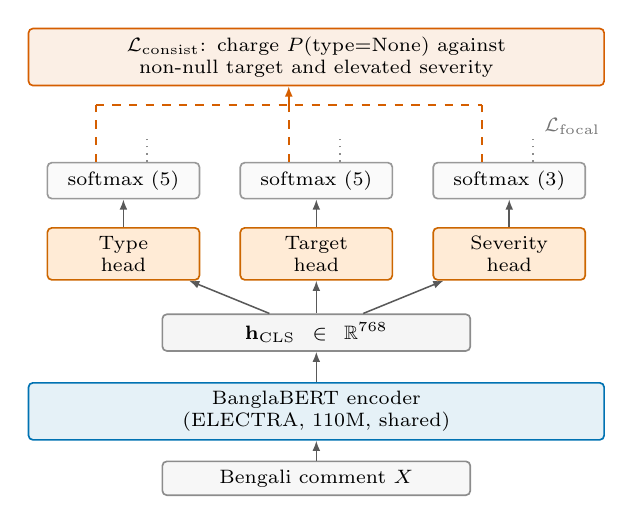
\begin{tikzpicture}[
  font=\scriptsize,
  blk/.style={draw, rounded corners=1.6pt, align=center,
              inner xsep=3pt, inner ysep=3pt, line width=0.6pt},
  io/.style   ={blk, fill=black!3,  draw=black!45, text width=3.7cm},
  enc/.style  ={blk, fill=cUnc!10,  draw=cUnc,     text width=7.1cm},
  pool/.style ={blk, fill=black!4,  draw=black!45, text width=3.7cm},
  head/.style ={blk, fill=orange!16,draw=orange!80!black, text width=1.72cm},
  sm/.style   ={blk, fill=black!2,  draw=black!40, text width=1.72cm},
  cons/.style ={blk, fill=cCon!10,  draw=cCon,     text width=7.1cm},
  ar/.style   ={-{Latex[length=1.3mm,width=1.0mm]}, draw=black!65, line width=0.55pt},
  bus/.style  ={draw=cCon, dashed, line width=0.6pt},
  foc/.style  ={draw=black!45, dotted, line width=0.6pt},
]
\node[io]   (in)   at (0,0)      {Bengali comment $X$};
\node[enc]  (enc)  at (0,0.85)   {BanglaBERT encoder\\(ELECTRA, 110M, shared)};
\node[pool] (cls)  at (0,1.85)   {$\mathbf{h}_{\text{CLS}} \in \mathbb{R}^{768}$};

\node[head] (h1) at (-2.45,2.85) {Type\\head};
\node[head] (h2) at (0,2.85)     {Target\\head};
\node[head] (h3) at (2.45,2.85)  {Severity\\head};

\node[sm] (s1) at (-2.45,3.78) {softmax (5)};
\node[sm] (s2) at (0,3.78)     {softmax (5)};
\node[sm] (s3) at (2.45,3.78)  {softmax (3)};

\node[cons] (co) at (0,5.35)
  {$\mathcal{L}_{\text{consist}}$: charge $P(\text{type}{=}\text{None})$ against\\
   non-null target and elevated severity};

\draw[ar] (in)  -- (enc);
\draw[ar] (enc) -- (cls);
\foreach \h in {h1,h2,h3}{\draw[ar] (cls) -- (\h);}
\draw[ar] (h1) -- (s1);
\draw[ar] (h2) -- (s2);
\draw[ar] (h3) -- (s3);

% focal loss: applied independently to each head, so no shared bus
\foreach \s in {s1,s2,s3}{\draw[foc] ($(\s.north)+(0.30,0)$) -- ++(0,0.34);}
\node[anchor=south west, font=\scriptsize, text=black!55, inner sep=1pt]
  at ($(s3.north)+(0.40,0.30)$) {$\mathcal{L}_{\text{focal}}$};

% consistency bus
\foreach \s in {s1,s2,s3}{\draw[bus] ($(\s.north)+(-0.35,0)$) -- ++(0,0.72);}
\draw[bus] ($(s1.north)+(-0.35,0.72)$) -- ($(s3.north)+(-0.35,0.72)$);
\draw[ar, draw=cCon] ($(s2.north)+(-0.35,0.72)$) -- ($(co.south)+(-0.35,0)$);
\end{tikzpicture}
\caption{The model. Focal loss (dotted) is applied to each head
independently. The consistency penalty (dashed) is the only path that
couples the three softmax outputs, so a contradiction is paid for during
backpropagation rather than repaired at inference.}
\label{fig:arch}
\end{figure}

\subsection{Objective}
The label distribution is badly skewed, with Gender Hate at 0.34 percent of the corpus, so each head is trained with multi-class focal loss \cite{lin2017focal},
\begin{equation}
\mathcal{L}_{\text{focal}}^t = -\frac{1}{N} \sum_{i=1}^N \alpha_{y_i^t} \left(1 - P(y_i^t \mid X_i)\right)^\gamma \log P(y_i^t \mid X_i)
\end{equation}
with $\gamma = 2.0$ and $\alpha_c = N / (K n_c)$ set inversely to class frequency.

For the constraint, write $\pi_i = P_i(\text{type}{=}\text{None})$ for the mass the model puts on the comment being harmless, and let $\tau_i = P_i(\text{target}{=}\text{None})$, $\sigma_i = P_i(\text{sev}{=}\text{Little to None})$ and $\varsigma_i = P_i(\text{sev}{=}\text{Severe})$. Then
\begin{equation}
\mathcal{L}_{\text{consist}} = \frac{1}{N} \sum_{i=1}^{N} \pi_i \left[ (1 - \tau_i) + (1 - \sigma_i) + 2\,\varsigma_i \right]
\label{eq:consist}
\end{equation}
The first two terms are \eqref{eq:rule} written in probabilities: whatever mass sits on $\text{type}=\text{None}$ is multiplied by the mass that sits, illegally, on a non-null target or an elevated severity. The third term charges the worst case twice over, a comment called harmless and severe in the same breath. We added it after observing that severity contradictions were what remained once the target contradictions had been suppressed. The whole term is zero exactly when belief in $\text{type}=\text{None}$ coincides with belief in $\text{target}=\text{None}$ and $\text{sev}=\text{Little to None}$, and it is differentiable everywhere.

Training minimises
\begin{equation}
\mathcal{L}_{\text{total}} = \mathcal{L}_{\text{focal}}^{\text{type}} + \mathcal{L}_{\text{focal}}^{\text{target}} + \mathcal{L}_{\text{focal}}^{\text{sev}} + \lambda \, \mathcal{L}_{\text{consist}}
\end{equation}
Switching the penalty on at full strength from step one does not work. Early in training the heads are close to uniform, every example looks like a violation, and the gradient from \eqref{eq:consist} swamps the classification signal. We ramp $\lambda$ linearly from $0.01$ to $1.0$ across the ten epochs. Unconstrained runs hold $\lambda = 0$ throughout.

\section{Experimental Setup}
\label{sec:exp}

\subsection{Data}
We use the BanglaMultiHate training corpus \cite{hasan2026banglamultihate}: 35{,}522 Bengali comments annotated from YouTube, Facebook and news-site discussion. The original type inventory keeps \emph{Profane} and \emph{Abusive} apart. In Bengali the two overlap almost completely at the lexical level, and separating them mostly measures annotator preference, so we merge Profane into Abusive. We also rename \emph{Sexism} to \emph{Gender Hate}, which better fits the range of examples actually annotated under it. Target and severity labels are untouched. Table~\ref{tab:data} gives the result. The ground truth satisfies \eqref{eq:rule} exactly: not one comment labelled $\text{type}=\text{None}$ carries a non-null target or an elevated severity.

\begin{table}[t]
\caption{Label distribution over the 35{,}522-comment corpus, after merging
Profane into Abusive and renaming Sexism to Gender Hate}
\label{tab:data}
\centering
\footnotesize
\begin{tabular}{llrr}
\toprule
\textbf{Dimension} & \textbf{Class} & \textbf{Count} & \textbf{Share} \\
\midrule
\multirow{5}{*}{Hate Type}
& None            & 19{,}954 & 56.17\% \\
& Abusive         & 10{,}543 & 29.68\% \\
& Political Hate  & 4{,}227  & 11.90\% \\
& Religious Hate  & 676      & 1.90\%  \\
& Gender Hate     & 122      & 0.34\%  \\
\midrule
\multirow{5}{*}{Target}
& None            & 21{,}190 & 59.65\% \\
& Individual      & 5{,}646  & 15.89\% \\
& Organization    & 3{,}846  & 10.83\% \\
& Community       & 2{,}635  & 7.42\%  \\
& Society         & 2{,}205  & 6.21\%  \\
\midrule
\multirow{3}{*}{Severity}
& Little to None  & 23{,}489 & 66.13\% \\
& Mild            & 6{,}853  & 19.29\% \\
& Severe          & 5{,}180  & 14.58\% \\
\bottomrule
\end{tabular}
\end{table}

\subsection{Partitioning}
The corpus is split 80/10/10 with seed 42, stratified on hate type, giving 28{,}417 training, 3{,}552 validation and 3{,}553 test comments. Every downstream stage regenerates the split deterministically from that seed, so training, evaluation and LLM benchmarking all address the same held-out comments. Validation is used for checkpoint selection and nothing else. No model sees a test comment during training, and the 5-shot demonstrations given to the LLMs are held out of the test split.

\subsection{Training}
All runs fine-tune \texttt{csebuetnlp/banglabert} for ten epochs with AdamW \cite{loshchilov2017decoupled}, weight decay 0.01, batch size 16 and maximum sequence length 256. The encoder and the heads get different learning rates, $2 \times 10^{-5}$ and $1 \times 10^{-4}$, with linear warmup over the first 10 percent of steps and gradient-norm clipping at 1.0. We keep the checkpoint with the best validation average macro F1 and stop early after five epochs without improvement. Training used a single NVIDIA Tesla T4.

We train two configurations, unconstrained ($\lambda = 0$) and constrained ($\lambda: 0.01 \rightarrow 1.0$), and run each twice. The two runs of a configuration differ in random initialisation. They are not byte-identical replicates: run~B of each configuration was produced by a training script that also instantiates an auxiliary sequence-decoder module. That module never enters the classification forward pass and never receives a gradient, so it changes run~B only by consuming random draws at construction time and thereby shifting the initialisation of the heads and the data-shuffling order. We treat the four runs as two initialisations per configuration. Two runs will not support a significance test, but they are enough to show that run-to-run variance on this dataset is large enough to mislead a single-run comparison, which turns out to matter for one of our results. All parameter counts and the headline results in Table~\ref{tab:llm} refer to run~A, the 110M encoder-plus-heads model with no auxiliary module.

\subsection{LLM Baselines}
We evaluate three published Bengali LLMs in half precision on the same T4: TigerLLM-1B-it \cite{raihan2025tigerllm} (checkpoint \texttt{md-nishat-008/TigerLLM-1B-it}), TituLM-1B \cite{hishab2024titullm} (\texttt{hishab/titulm-llama-3.2-1b-v2.0}), and BanglaLLama-3.2-3B \cite{banglallm2024bongllama} (\texttt{BanglaLLM/BanglaLLama-3.2-3b-bangla-alpaca-orca-instruct-v0.0.1}), the last two being instruction-tuned adaptations of Llama 3.2 \cite{touvron2023llama}. Prompts are written in Bengali, list the three label inventories, and ask for one JSON object with keys \texttt{type\_of\_hate}, \texttt{target\_of\_hate} and \texttt{severity\_of\_hate}. The 5-shot variant prepends five fixed demonstrations, one per hate type; none of them appears in the test split. Generation is capped at 64 new tokens.

Responses are parsed by decoding the first brace-delimited span as JSON, falling back to line-wise key extraction. A response yielding no recoverable label counts as a parse failure. Macro F1 needs a prediction for every example, so the harness substitutes the majority triple (None, None, Little to None) whenever parsing fails. This is ordinary practice and it has a consequence we return to in Section~\ref{sec:llm}: as the parse rate falls, the reported F1 converges on the constant majority-class baseline and stops describing the model at all.

\section{Results}
\label{sec:results}

\subsection{What the Constraint Does}
Table~\ref{tab:ablation} gives both runs of both configurations on the 3{,}553 held-out comments, and Fig.~\ref{fig:dyn} tracks them across training.

\begin{table}[t]
\caption{Held-out test results, two runs per configuration ($n = 3{,}553$).
The two runs differ in initialisation; run~B additionally carries the
inactive module described in Section~\ref{sec:exp}, which does not touch the
classification path.}
\label{tab:ablation}
\centering
\footnotesize
\setlength{\tabcolsep}{3.4pt}
\begin{tabular}{llccccrr}
\toprule
\textbf{Config.} & \textbf{Run} & \textbf{Type} & \textbf{Target} & \textbf{Sev.} & \textbf{Avg F1} & \textbf{CVR} & \textbf{Viol.} \\
\midrule
\multirow{3}{*}{Unconstrained}
 & A & 0.5111 & 0.5109 & 0.5972 & 0.5397 & 9.46\% & 336 \\
 & B & 0.5270 & 0.5228 & 0.5988 & 0.5495 & 4.95\% & 176 \\
 & mean & 0.5191 & 0.5169 & 0.5980 & 0.5446 & 7.21\% & 256.0 \\
\midrule
\multirow{3}{*}{Constrained}
 & A & 0.4959 & 0.5652 & 0.6110 & 0.5574 & 0.00\% & 0 \\
 & B & 0.4994 & 0.5598 & 0.6136 & 0.5576 & 0.03\% & 1 \\
 & mean & 0.4977 & \textbf{0.5625} & \textbf{0.6123} & \textbf{0.5575} & \textbf{0.015\%} & \textbf{0.5} \\
\bottomrule
\end{tabular}
\end{table}

\begin{figure*}[t]
\centering
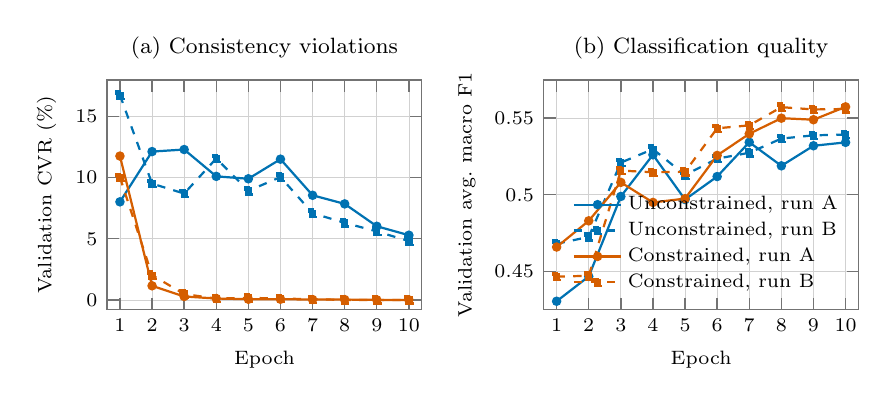
\begin{tikzpicture}
\begin{groupplot}[
  group style={group size=2 by 1, horizontal sep=1.55cm},
  paperaxis, width=0.46\textwidth, height=4.5cm,
  xlabel={Epoch}, xmin=0.6, xmax=10.4, xtick={1,...,10},
]
\nextgroupplot[ylabel={Validation CVR (\%)}, ymin=-0.8, ymax=18,
               title={\footnotesize (a) Consistency violations},
               title style={yshift=-2pt}]
\addplot[uA] coordinates {(1,8.0236)(2,12.1340)(3,12.3029)(4,10.1070)(5,9.9099)(6,11.5146)(7,8.5586)(8,7.8547)(9,6.0248)(10,5.2928)};
\addplot[uB] coordinates {(1,16.7511)(2,9.5158)(3,8.6993)(4,11.5709)(5,8.9245)(6,10.0507)(7,7.0946)(8,6.3063)(9,5.6025)(10,4.8142)};
\addplot[cA] coordinates {(1,11.7680)(2,1.1543)(3,0.2815)(4,0.1126)(5,0.0563)(6,0.0563)(7,0.0282)(8,0.0282)(9,0.0000)(10,0.0000)};
\addplot[cB] coordinates {(1,10.0225)(2,2.0270)(3,0.4786)(4,0.1126)(5,0.1689)(6,0.1126)(7,0.0563)(8,0.0000)(9,0.0000)(10,0.0000)};

\nextgroupplot[ylabel={Validation avg.\ macro F1}, ymin=0.425, ymax=0.575,
               title={\footnotesize (b) Classification quality},
               title style={yshift=-2pt},
               legend style={at={(0.98,0.03)}, anchor=south east},
               legend cell align=left]
\addplot[uA] coordinates {(1,0.4305)(2,0.4467)(3,0.4989)(4,0.5261)(5,0.4969)(6,0.5119)(7,0.5343)(8,0.5189)(9,0.5320)(10,0.5342)};
\addlegendentry{Unconstrained, run A}
\addplot[uB] coordinates {(1,0.4680)(2,0.4725)(3,0.5210)(4,0.5298)(5,0.5129)(6,0.5236)(7,0.5274)(8,0.5367)(9,0.5388)(10,0.5393)};
\addlegendentry{Unconstrained, run B}
\addplot[cA] coordinates {(1,0.4659)(2,0.4830)(3,0.5081)(4,0.4950)(5,0.4975)(6,0.5257)(7,0.5398)(8,0.5500)(9,0.5490)(10,0.5574)};
\addlegendentry{Constrained, run A}
\addplot[cB] coordinates {(1,0.4466)(2,0.4471)(3,0.5158)(4,0.5147)(5,0.5150)(6,0.5434)(7,0.5453)(8,0.5572)(9,0.5557)(10,0.5560)};
\addlegendentry{Constrained, run B}
\end{groupplot}
\end{tikzpicture}
\caption{Validation behaviour across training. Constrained runs fall below
0.5 percent CVR by epoch three and reach zero by epochs eight and nine; on a
linear axis they are indistinguishable from the floor, which is the point.
Unconstrained runs never settle, sitting between 4.8 and 12.3 percent after the
first epoch and as high as 16.8 percent within it. Panel (b) shows that this
costs nothing in classification quality: the constrained runs finish higher.}
\label{fig:dyn}
\end{figure*}

Three things stand out.

The constraint works. Violations drop from a mean of 256 to a mean of 0.5. One constrained run ends with none at all, the other with a single borderline case out of 3{,}553.

It is not paid for in accuracy. Average macro F1 goes from 0.5446 to 0.5575, a relative gain of 2.4 percent, concentrated in target ($+0.046$) and severity ($+0.014$). That is the pattern you would expect if the penalty is stripping out spurious targets and severities on comments the model already reads as harmless. Type F1 does fall, from 0.5191 to 0.4977. The mechanism is visible in \eqref{eq:consist}: mass on $\text{type}=\text{None}$ is what gets charged, so when the target and severity heads are confident of nullity the cheapest way to satisfy the penalty is to agree with them, and on genuinely hateful but weakly marked comments that costs type recall. We think the exchange is worth making. It is still an exchange, and we would rather state it than bury it.

It also makes training predictable. The two unconstrained runs differ by 0.0098 average F1 and by 160 violations, nearly a factor of two. The two constrained runs differ by 0.0002 and by one violation. Fig.~\ref{fig:dyn}(a) shows why: without the penalty, CVR wanders for ten epochs without converging, so which epoch the checkpoint selector happens to pick has a large say in the reported number. That is an unpleasant property for a system anyone intends to deploy, and the constraint removes it.

This last point is also our reason for reporting two runs rather than one. A single unconstrained baseline could have been quoted at 4.95 percent CVR or at 9.46 percent, and the choice would have moved the headline reduction by a factor of two without any change to the method.

\subsection{Against Bengali LLMs}
\label{sec:llm}
Table~\ref{tab:llm} puts the three prompted LLMs and our constrained model on the same test set. The ``Ours'' row is run A, the constrained model without the additional module carried by run B, so its parameter count is exactly the 110M of the encoder plus the three heads. The last row is the constant majority-class baseline, the score obtained by predicting (None, None, Little to None) for every comment and never looking at the text.

\begin{table*}[t]
\caption{Bengali LLMs and our model on the identical 3{,}553-comment held-out set.
Rows marked $\dagger$ have parse rates at which the reported F1 describes the
harness fallback rather than the model. Latencies are single-run wall-clock on
one T4; our four checkpoints span 0.0141--0.0155\,s and we quote 0.015\,s}
\label{tab:llm}
\centering
\footnotesize
\begin{tabular}{llcccccccc}
\toprule
\textbf{Model} & \textbf{Paradigm} & \textbf{Params} & \textbf{Parse rate} & \textbf{Type F1} & \textbf{Target F1} & \textbf{Sev.\ F1} & \textbf{Avg macro F1} & \textbf{CVR} & \textbf{Latency} \\
\midrule
TigerLLM-1B-it \cite{raihan2025tigerllm} & 0-shot & 1B & 95.6\% & 0.2256 & 0.1851 & 0.3557 & 0.2554 & 0.42\% & 4.634\,s \\
TigerLLM-1B-it \cite{raihan2025tigerllm} & 5-shot & 1B & 99.1\% & 0.3572 & 0.2591 & 0.3747 & 0.3303 & 1.32\% & 5.851\,s \\
TituLM-1B \cite{hishab2024titullm} & 0-shot & 1B & 5.7\%$^\dagger$ & 0.1439 & 0.1500 & 0.2631 & 0.1856 & 0.00\% & 2.173\,s \\
TituLM-1B \cite{hishab2024titullm} & 5-shot & 1B & 21.5\%$^\dagger$ & 0.1803 & 0.1731 & 0.3014 & 0.2183 & 4.98\% & 5.274\,s \\
BanglaLLama-3.2-3B \cite{banglallm2024bongllama} & 0-shot & 3B & 0.0\%$^\dagger$ & 0.1439 & 0.1500 & 0.2631 & 0.1856 & 0.00\% & 0.218\,s \\
BanglaLLama-3.2-3B \cite{banglallm2024bongllama} & 5-shot & 3B & 100.0\% & 0.1439 & 0.1500 & 0.0844 & 0.1261 & 100.00\% & 1.277\,s \\
\midrule
\textbf{Ours (constrained, run A)} & Deterministic & \textbf{110M} & \textbf{100.0\%} & \textbf{0.4959} & \textbf{0.5652} & \textbf{0.6110} & \textbf{0.5574} & \textbf{0.00\%} & \textbf{$\sim$0.015\,s} \\
\midrule
Constant majority-class baseline & --- & --- & --- & 0.1439 & 0.1500 & 0.2631 & 0.1856 & 0.00\% & --- \\
\bottomrule
\end{tabular}
\end{table*}

\subsubsection{Two of the three baselines cannot be measured}
TigerLLM returns parseable JSON for 95.6 percent of zero-shot and 99.1 percent of 5-shot prompts, so its scores mean what they appear to mean. The other two do not. TituLM's zero-shot F1 of 0.1856 matches the constant baseline in all three dimensions, which follows directly from a 5.7 percent parse rate: almost every number in that row was produced by the fallback rule, not by the model. BanglaLLama's zero-shot parse rate is 0.0 percent, so its row \emph{is} the constant baseline, digit for digit. We report both rows to document the failure, not as measurements. For anyone building a moderation pipeline the useful finding here is about reliability rather than accuracy: two of three Bengali LLMs could not be trusted to return a parseable label triple at all.

\subsubsection{BanglaLLama degenerates under few-shot prompting}
The 5-shot BanglaLLama row is the interesting one, because parse rate and quality come apart completely. Every response parsed. Yet type F1 and target F1 land exactly on the all-None constants, 0.1439 and 0.1500, and severity F1 lands exactly on the all-Severe constant, 0.0844. Only one prediction pattern satisfies all three at once: a single invariant triple, (None, None, Severe), returned for all 3{,}553 comments. That triple violates \eqref{eq:rule} by construction, which is why CVR is exactly 100 percent and not merely high. The demonstrations taught the model the shape of the output and nothing about the task. We infer this from the metrics rather than from stored generations, since per-sample outputs were not retained; recovering them needs only a re-run of the benchmark.

\subsubsection{Cost}
Our model labels a comment in about 0.015 seconds against 5.851 for TigerLLM's better setting, a factor of roughly 390, and scores 68.8 percent higher in relative average macro F1 (0.5574 against 0.3303). At 110M parameters it runs on hardware a university lab already owns. For a moderation queue of any realistic size that gap decides the question on its own, before accuracy is considered.

\subsection{Rationale Faithfulness}
We apply ERASER \cite{deyoung2020eraser} to 1{,}000 test comments. A rationale is the top-$k$ tokens by mean $[\text{CLS}]$ attention in the encoder's final layer, for $k \in \{5, 10, 20, 50\}$ percent of non-special tokens; comments with five or fewer such tokens are skipped. Comprehensiveness replaces those tokens with the mask token and measures how far the predicted type probability falls. Sufficiency keeps only the rationale and measures the same fall. AOPC averages comprehensiveness over the four thresholds.

\begin{table}[t]
\caption{ERASER faithfulness on 1{,}000 test comments}
\label{tab:eraser}
\centering
\footnotesize
\begin{tabular}{llccc}
\toprule
\textbf{Config.} & \textbf{Run} & \textbf{Comp.@20\%} $\uparrow$ & \textbf{Suff.@50\%} $\downarrow$ & \textbf{AOPC} $\uparrow$ \\
\midrule
\multirow{3}{*}{Unconstrained}
 & A & 0.1443 & 0.0989 & 0.1430 \\
 & B & 0.1669 & 0.1059 & 0.1646 \\
 & mean & 0.1556 & 0.1024 & 0.1538 \\
\midrule
\multirow{3}{*}{Constrained}
 & A & \textbf{0.1746} & 0.1169 & \textbf{0.1752} \\
 & B & 0.1645 & \textbf{0.0745} & 0.1704 \\
 & mean & \textbf{0.1695} & \textbf{0.0957} & \textbf{0.1728} \\
\bottomrule
\end{tabular}
\end{table}

\begin{figure}[t]
\centering
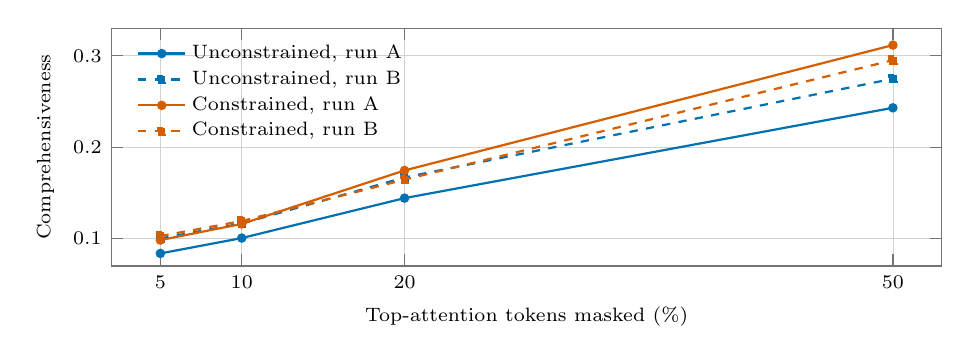
\begin{tikzpicture}
\begin{axis}[
  paperaxis, width=\linewidth, height=4.6cm,
  xlabel={Top-attention tokens masked (\%)},
  ylabel={Comprehensiveness},
  xmin=2, xmax=53, xtick={5,10,20,50},
  ymin=0.07, ymax=0.33,
  legend style={at={(0.02,0.98)}, anchor=north west},
  legend cell align=left,
]
\addplot[uA] coordinates {(5,0.0838)(10,0.1006)(20,0.1443)(50,0.2431)};
\addlegendentry{Unconstrained, run A}
\addplot[uB] coordinates {(5,0.1002)(10,0.1165)(20,0.1669)(50,0.2749)};
\addlegendentry{Unconstrained, run B}
\addplot[cA] coordinates {(5,0.0984)(10,0.1161)(20,0.1746)(50,0.3117)};
\addlegendentry{Constrained, run A}
\addplot[cB] coordinates {(5,0.1028)(10,0.1192)(20,0.1645)(50,0.2952)};
\addlegendentry{Constrained, run B}
\end{axis}
\end{tikzpicture}
\caption{Comprehensiveness against the fraction of top-attention tokens
masked. Constrained runs sit above unconstrained ones across the range,
though the two dashed curves nearly touch at 20 percent, which is where the
effect is weakest.}
\label{fig:perturb}
\end{figure}

Table~\ref{tab:eraser} and Fig.~\ref{fig:perturb} give the results. Constrained models are more faithful on average: AOPC rises from 0.1538 to 0.1728, a relative gain of 12.4 percent, and mean comprehensiveness at 20 percent rises from 0.1556 to 0.1695. Deleting the tokens a constrained encoder attends to hurts its prediction more than the same operation hurts an unconstrained one, which is the behaviour a faithful rationale should show.

The effect is uneven. Pairing run A against run A gives 22.6 percent; pairing B against B gives 3.5 percent. We report the mean rather than the flattering pair, and we would not want the 12.4 percent read as a precise quantity. Sufficiency is noisier again: the best constrained run posts the lowest score in the table, 0.0745, and the other constrained run posts the worst, 0.1169. We draw no conclusion from that column.

\section{Limitations}
\label{sec:limits}
Two runs per configuration establishes that variance is worth worrying about and keeps us from over-reading a single pairing. It does not support a significance test. The ERASER result in particular should be read as suggestive; the classification and CVR results are separated by margins far larger than the observed spread, and we are correspondingly more confident in them.

The rule in \eqref{eq:rule} belongs to this taxonomy and points one way. We have not tested whether the same construction extends to richer dependency graphs, or to constraints that annotators themselves apply inconsistently.

Our LLM comparison is against prompting, not against fine-tuning. A fine-tuned 1B Bengali model would be a harder baseline and we do not offer one; the claim we support is about prompted structured output, which is how these models are usually reached for. Prompts were not tuned per model beyond the zero-shot and 5-shot forms, and decoding used temperature 0.1 with sampling on rather than greedy decoding, so a small amount of sampling noise sits in the LLM numbers. We did not store per-sample generations, which is why we cannot report F1 restricted to parsed responses. That restricted figure is the more informative one and we intend to report it next.

Finally, the drop in type F1 under the constraint is real, and we have not established which kinds of comment account for it.

\section{Conclusion}
We treated multi-aspect Bengali hate speech detection as a constrained joint prediction, and showed that charging a model for probability mass on contradictory label combinations removes essentially all of its logical violations, from a mean of 256 to 0.5 out of 3{,}553 held-out comments, while raising average macro F1 from 0.5446 to 0.5575. The constraint also collapses the run-to-run spread, which matters more for deployment than the headline average does.

Set against prompted Bengali LLMs, a 110M-parameter constrained model beats the strongest baseline by 68.8 percent relative macro F1 at roughly 390 times the throughput. Two of the three LLMs never produced parseable structured output often enough to be scored at all, and the harness quietly filled the gap with a majority-class guess. That is the finding we would most like other groups to take up: in a low-resource language, format reliability is a precondition for evaluation, and an aggregate F1 reported without a parse rate beside it can be almost entirely an artefact of the scoring code.

\section*{Acknowledgment}
The authors thank the providers of the computing resources used to train and evaluate the models described here.

\bibliographystyle{IEEEtran}
\bibliography{references}

\end{document}
